\chapter{Plasma Models}

	\section{\texttt{spicedmodel}: The Scalable Plasma Ion Composition and Electron Density Model}



	\section{\texttt{spiced}}

	\section{\texttt{HermeanFLRModel}: Model of Mercury's dayside plasma mass density}

	\section{\texttt{PyGCPM}: Wrapper for the Global Core Plasma Model}
	
		GitHub: \href{https://github.com/mattkjames7/PyGCPM.git}{https://github.com/mattkjames7/PyGCPM.git}

		This is a Python wrapper for the Global Core Plasma Model (\citet{Gallagher2000}, \href{https://plasmasphere.nasa.gov/models/}{code found here})

		\subsection{Installation}

			This module exists on PyPI, so can be installed using \texttt{pip}:
			\begin{minted}{bash}
pip3 install PyGCPM --user
			\end{minted}

		\subsection{Usage}

			There are three functions:
			\begin{enumerate}
				\item \texttt{PyGCPM.GCPM()}: provides particle densities at positions defined in SM coordinates.
				\item \texttt{PyGCPM.PlotEqSlice()} : plots the density of a species in the equatorial plane.
				\item \texttt{PyGCPM.PlotMLTSlice()} : plots the density of a particle species in 
			\end{enumerate}

			Firstly, get some densities at some positions in SM coordinates, units of $R_E$:
			\begin{minted}{python}
import PyGCPM
ne,nH,nHe,nO = PyGCPM.GCPM(x,y,z,Date,ut,Kp=Kp,Verbose=Verbose)
			\end{minted}
			where \texttt{Date} is the date in the format yyyymmdd, \texttt{ut} is the time in hours, \texttt{Kp} is the Kp index and \texttt{Verbose=True} would display progress. The outputs of this function \texttt{ne}, \texttt{nH}, \texttt{nHe} and \texttt{nO} are the densities of electrons, protons, helium ions and oxygen ions, respectively.

			We can plot the density of a particle species in the equatorial plane:
			\begin{minted}{python}
PyGCPM.PlotEqSlice(20010902,12.0,Parameter='ne')
			\end{minted}
			which should produce the plot in figure \ref{FigPyGCPMEq}.

			\begin{figure}
				\begin{center}
					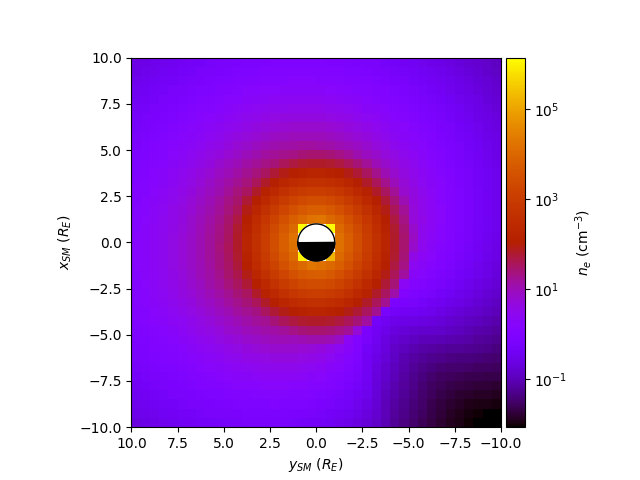
\includegraphics[width=0.8\textwidth]{figures/ch2_pygcpm_equator.png}
				\end{center}
				\caption{Equatorial electon density. \label{FigPyGCPMEq}}
			\end{figure}

			We can also plot the density of a particle species in a slice of MLT:
			\begin{minted}{python}
PyGCPM.PlotMLTSlice(8.0,20010902,12.0,Parameter='ne')
			\end{minted}
			which should produce the plot in figure \ref{FigPyGCPMMLT}.

			\begin{figure}
				\begin{center}
					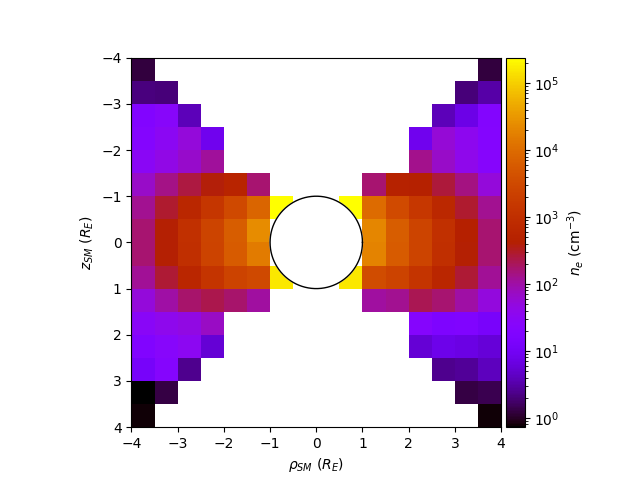
\includegraphics[width=0.8\textwidth]{figures/ch2_pygcpm_mlt.png}
				\end{center}
				\caption{MLT slice of electon density. \label{FigPyGCPMMLT}}
			\end{figure}